\chapter{推論統計:區間估計}

    統計中對於未知參數的估計方法有兩種:\textit{點估計} (point estimation) 和\textit{區間估計} (interval estimation)。其中點估計較為直觀,即利用樣本求出一個統計量(稱為估計量)來估計未知參數。我們在第二章已經提到了針對母體平均與母體變異數的最佳點估計量(即樣本平均與樣本變藝術),並在第四章中提到評估點估計量時需要知道估計量的抽樣分布,以了解該估計量是否不偏,以及該估計量的標準誤多大。
    
    在這一章,我們將會深入探討參數的另一類估計方法:區間估計。我們將從平均值區間估計的建構方式出發,了解樣本平均的抽樣分布在區間估計扮演的角色,以及如何正確解釋區間估計隱含的機率敘述。
    
    \begin{introduction}[第 \thechapter 章學習目標]
        \item 了解估計的兩種型式:點估計和區間估計
        \item 了解信賴區間的解釋意義
        \item 計算母體為常態分布下平均值的信賴區間
        \item 計算母體為其他分布下平均值的信賴區間
    \end{introduction}

    點估計是用一個數值來估計母體參數,因此我們需要額外用估計值的標準誤來量化點估計的不確定性。區間估計則是利用區間來估計參數,例如「我們有 95\% 的信心,清華大學生的平均身高將被 (160, 170) 公分這個區間覆蓋。」這樣的估計方法雖然沒有明確指出一個估計值,但是同時告知了估計的約略位置以及不確定性,因此被稱為區間估計。
    
    建構區間估計的其中一種方法是先尋找一個含未知參數、但分布已知的量(這在統計中被稱為樞紐量 (pivotal quantity))。例如,如果我們在某種狀況下已知清華大學生的身高標準差為 5 公分,但是不知道母體平均值為何。這時候我們抽了 36 位學生得到平均身高為 $\bar{X}$ 公分,則根據前一章所述,若母體平均值為 $\mu$ 公分,則 $\bar{X}$ 的抽樣分布為
    \[\bar{X} \sim \NN\Big(\mu, \frac{5^2}{36}\Big)\]
    此時可以發現,將 $\bar{X}$ 作 z 轉換,就可以得到一個服從標準常態分布的樞紐量:
    \[\frac{\bar{X} - \mu}{5/\sqrt{36}} \sim \ZZ\]
    如果我們此時想得到 $95\%$ 信心的區間估計,可以先從以下的等式出發,建構出一個以 0 為中心左右對稱,且機率為 $95\%$ 的區間:
    \[\PP(-z_{0.025} < \ZZ < z_{0.025}) = 1-2 \times 0.025 = 0.95\]
    其中 $z_{0.025}$ 是已知的數值,大約是\textbf{1.96},可以用查表得到。根據前面樞紐量的分布,我們可以推出:
    \begin{align*}
        \PP\Big(-z_{0.025} < \frac{\bar{X} - \mu}{5/\sqrt{36}} < z_{0.025}\Big) &= 0.95\\
        \PP\Big(-z_{0.025}\cdot \frac{5}{6} < \bar{X} - \mu < z_{0.025}\cdot \frac{5}{6}\Big) &= 0.95\\
        \PP\Big(\bar{X}-z_{0.025}\cdot \frac{5}{6} < \mu < \bar{X} + z_{0.025}\cdot \frac{5}{6}\Big) &= 0.95\\
        \PP\Big(\mu \in \Big(\bar{X}-z_{0.025}\cdot \frac{5}{6},  \bar{X} + z_{0.025}\cdot \frac{5}{6}\Big)\Big) &= 0.95
    \end{align*}
    上述的式子代表,在母體服從 $\NN(\mu, 5^2)$ 的假設下,如果我們重複抽取 36 位學生,並把每次得到的平均身高 $\bar{X}$ 都拿來算出一個區間 $\big(\bar{X}-z_{0.025}\cdot \frac{5}{6},  \bar{X} + z_{0.025}\cdot \frac{5}{6}\big)$,那麼這個區間覆蓋到 $\mu$ 的機率為 $95\%$。以圖\ref{fig:confidence_interval}為例,當$\mu = 160$時,重複抽取 36 人 200 次得到的 200 個區間中,僅有 10 個未蓋到 $160$ (在圖中以紅色標示),即蓋到的機率為 $190/200 = 95\%$。區間計算方式滿足上述性質時,我們稱\textbf{$\big(\bar{X}-z_{0.025}\cdot \frac{5}{6},  \bar{X} + z_{0.025}\cdot \frac{5}{6}\big)$是$\mu$ 的 95\% 信賴區間}。而因為這個信賴區間同時具有上下限,我們也常稱這種信賴區間為\textit{雙尾信賴區間}。
    
    \begin{figure}[htbp]
        \centering
        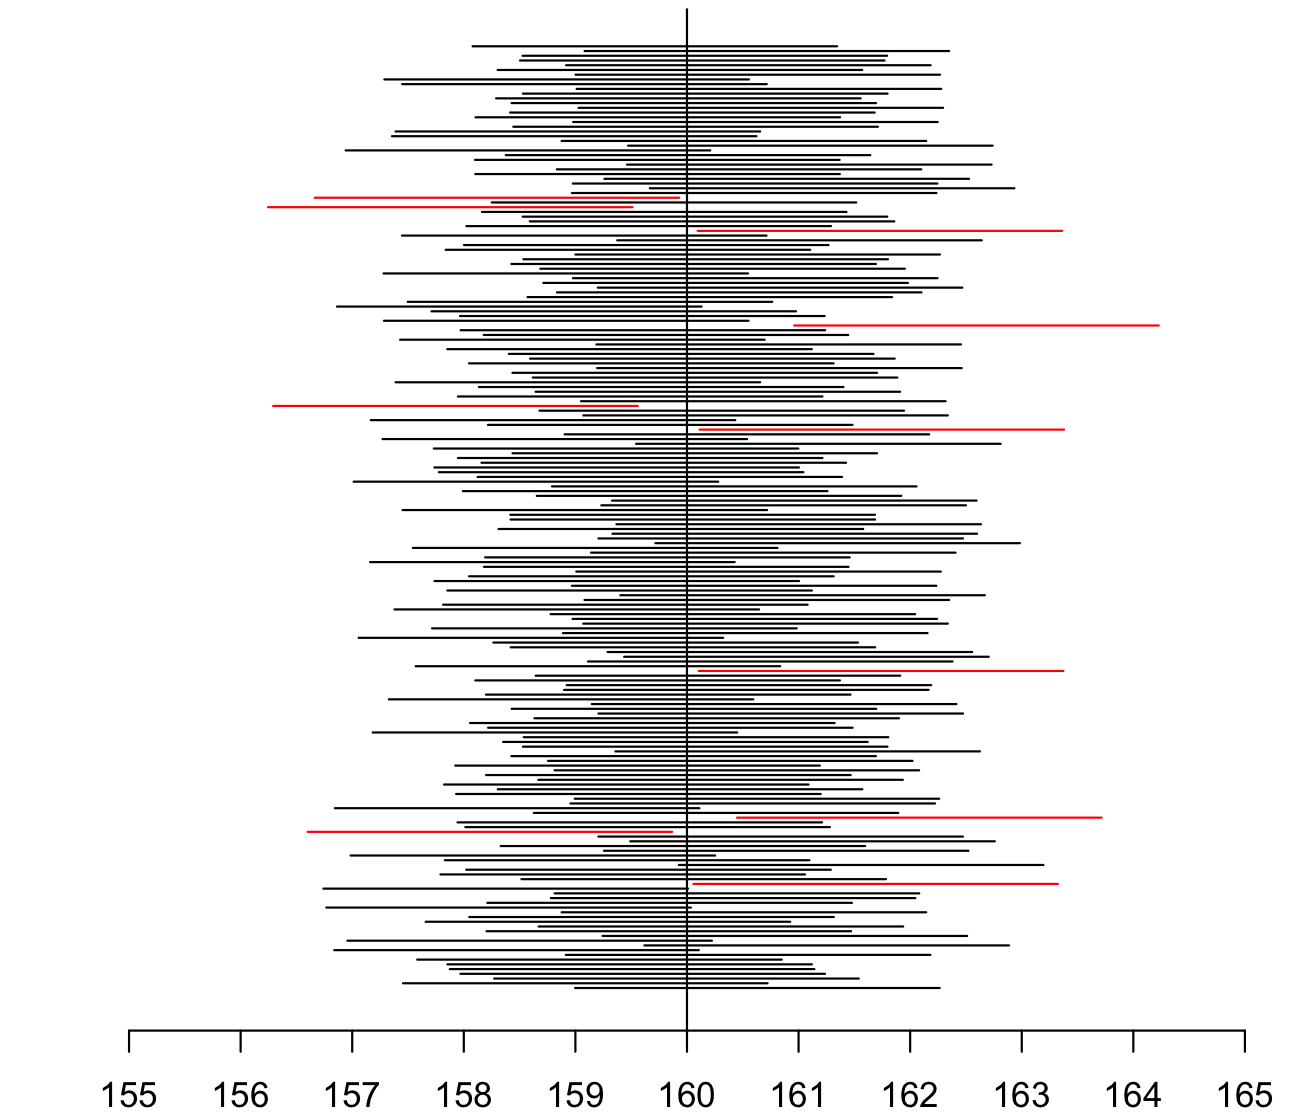
\includegraphics[width=0.7\textwidth]{figures/05-Confidence_interval/Confidence_interval.png}
        \caption{從 $\NN(160, 5^2)$ 抽出樣本數 36 的 200 組樣本,所得到的200個平均值 95\% 信賴區間}
        \label{fig:confidence_interval}
    \end{figure}
    
    注意到上述信賴區間性質的定義中,隨著每次抽樣,$\bar{X}$會有所變動,因此\textbf{整個區間會隨著抽樣而有不確定性}。這個「區間具有不確定性」的觀念可以衍生出兩個重點:
    \begin{itemize}
        \item 信賴區間的機率是針對「產生信賴區間的算法」而非觀察到的信賴區間數值:我們抽得一個樣本後,可以根據該樣本的觀察值算出一個區間(即圖 \ref{fig:confidence_interval}中的其中一條橫線)。但這個區間只是眾多可能的區間中被抽樣出來的一個,而信賴區間裡的 $95\%$ 是針對整體可能的區間作的機率性描述,而不是針對單一的區間觀察值。
        \item 參數雖未知但不具變動性,區間才有抽樣造成的變動性:前面我們在描述 $\PP\big(\mu \in \big(\bar{X}-z_{0.025}\cdot \frac{5}{6},  \bar{X} + z_{0.025}\cdot \frac{5}{6}\big)\big)$ 時,不用 $\mu$ 「落在」區間的機率,而是用區間「覆蓋」$\mu$ 的機率,即為強調 $\mu$ 本身不動,是區間在隨著抽樣而變動的概念。
    \end{itemize}
    前面我們用了一些實際數字來演示信賴區間的建構方法。利用符號來一般性地說明的話,假設母體來自於已知標準差為 $\sigma$ 的常態分佈,且 $\bar{X}$ 為樣本數 $n$ 的樣本算出的樣本平均,則母體平均值的 $(1-\alpha) \times 100\%$ 雙尾信賴區間可寫為
    \[\Big(\bar{X}-z_{\alpha/2}\frac{\sigma}{\sqrt{n}},  \bar{X} + z_{\alpha/2}\frac{\sigma}{\sqrt{n}}\Big)\]
    可以看到,這個雙尾區間以樣本平均 $\bar{X}$ 為中心,左右的寬度則各為 $z_{\alpha/2}\frac{\sigma}{\sqrt{n}}$。寬度取決於三個因子:
    \begin{itemize}
        \item 母體標準差 $\sigma$:母體的標準差越大,信賴區間的寬度越寬,意味著估計的不確定度越高。
        \item 樣本數 $n$:樣本數越大,信賴區間的寬度越窄,意味著估計越精準。
        \item 信賴區間的覆蓋率 $1-\alpha$:覆蓋率越高,$\alpha$越小,$z_{\alpha/2}$的值就越大,信賴區間的寬度就越寬。意即要提高覆蓋率,就要把信賴區間拉寬作為代價。
    \end{itemize}
    若我們有興趣的是單尾的信賴區間,則可以利用 $\PP(\ZZ > -z_{\alpha}) = \PP(\ZZ < z_{\alpha}) = 1-\alpha$ ,以相同的推導方式建立出下列右尾和左尾$(1-\alpha) \times 100\%$信賴區間:
    \[\Big(\bar{X}-z_{\alpha}\frac{\sigma}{\sqrt{n}},  \infty\Big), \;\;\Big(-\infty,  \bar{X} + z_{\alpha}\frac{\sigma}{\sqrt{n}}\Big)\]
    
    \begin{custom}{思考}
       在這個常態分布的例子中,如果要讓平均值信賴區間的覆蓋機率達到 100 \%,那麼寬度會變成多寬?
    \end{custom}

    \bigskip

    \begin{custom}{練習}
        假設已知 60 歲以上國人血清低密度脂蛋白的濃度標準差為 10 mg/dL,且呈現常態分布。現隨機選取 400 位 60 歲以上的志願者抽血,得到血清低密度脂蛋白的平均濃度為 93 mg/dL。請問 60 歲以上國人平均血清低密度脂蛋白濃度的 (1) 雙尾 95\% 信賴區間為何? (2) 右尾 90\% 信賴區間為何?
    \end{custom}

    \bigskip

    若母體並非來自常態分布,平均值信賴區間的建構較不直觀。然而,當樣本數夠大時,我們還有一個重要的法寶:中央極限定理!舉例來說,如果母體分布為機率參數為 $p$ 的白努利分布,那麼抽取樣本數為 $n$ 的樣本後,計算樣本中取值 1 的比例 $\hat{p}$ 相當於計算樣本平均值。根據中央極限定理:
    \[\hat{p} \xrightarrow{d} \NN\Big(p, \frac{p(1-p)}{n}\Big)\]
    所以利用類似常態分布的方法,我們可以構造以下關於 $p$ 的(近似) $(1-\alpha)\times 100\%$雙尾信賴區間
    \[\Big(\hat{p} - z_{\alpha/2} \sqrt{\frac{p(1-p)}{n}}, \hat{p} + z_{\alpha/2} \sqrt{\frac{p(1-p)}{n}}\Big)\]
    不過上面式子的問題是,根號中的 $p$ 仍是未知的參數,所以我們用 $p$ 最好的估計值 $\hat{p}$ 來取代 $p$,最終得到
    \[\Big(\hat{p} - z_{\alpha/2} \sqrt{\frac{\hat{p}(1-\hat{p})}{n}}, \hat{p} + z_{\alpha/2} \sqrt{\frac{\hat{p}(1-\hat{p})}{n}}\Big)\]
    這個公式也常被當成是比例信賴區間的通式。同樣地,右尾和左尾的(近似) $(1-\alpha)\times 100\%$單尾信賴區間為
    \[\Big(\hat{p} - z_{\alpha} \sqrt{\frac{\hat{p}(1-\hat{p})}{n}}, 1\Big), \;\; \Big(0, \hat{p} + z_{\alpha} \sqrt{\frac{\hat{p}(1-\hat{p})}{n}}\Big)\]
    此處左右尾的界線設定在 0 和 1,因為實際上的參數 $p$ 不可能超過 $[0,1]$ 的範圍。注意到這些近似信賴區間只有在 $n$ 夠大的時候,聲稱的 $(1-\alpha)\times 100\%$ 覆蓋率才會成立。一般而言,當 $np$ 及 $n(1-p)$ 均大於 $5$ 時,這個信賴區間的表現就已經很不錯。

    \bigskip
    
    \begin{custom}{練習}
        某大型醫療體系對員工進行血糖抽檢,隨機抽檢 160 人後發現,有 12 員工呈現空腹血糖過高的現象。請問該體系員工空腹血糖過高比率之 95\% 信賴區間為何?
    \end{custom}

    \bigskip

    \begin{custom}{練習}
        某民調公司希望藉由隨機電訪了解民眾對於 A 總統的支持度。若民調公司希望無論調查結果如何,最後建構出之支持度 95\% 雙尾信賴區間均不寬於上下 3\% (也就是總寬度不超過 6\%),那麼至少應收回多少有效電訪樣本?
    \end{custom}

    \bigskip

    前面我們針對常態分布的母體平均建立信賴區間時,作了一個不太常見的假設:母體標準差已知為。大部分的情況下,母體標準差都是未知的,因此雙尾信賴區間的公式就會多出一個未知數 $\sigma$。最直覺的解決辦法是直接參考比例信賴區間的做法,用樣本標準差帶入 $\sigma$,但這個方法在 $n$ 不夠大時,樣本標準差估計的準確度不佳,會造成整體的信賴區間覆蓋率不足。舉例來說,圖\ref{fig:confidence_t}中,假設母體和圖\ref{fig:confidence_interval}一樣服從 $\NN(160, 5^2)$,但是樣本數只有 9,且我們使用前述的雙尾 95\% 信賴區間公式並把 $\sigma$ 帶入樣本標準差,則 200 個平均值信賴區間中,有高達 18 個沒有覆蓋到正確值 160!

    \begin{figure}[htbp]
        \centering
        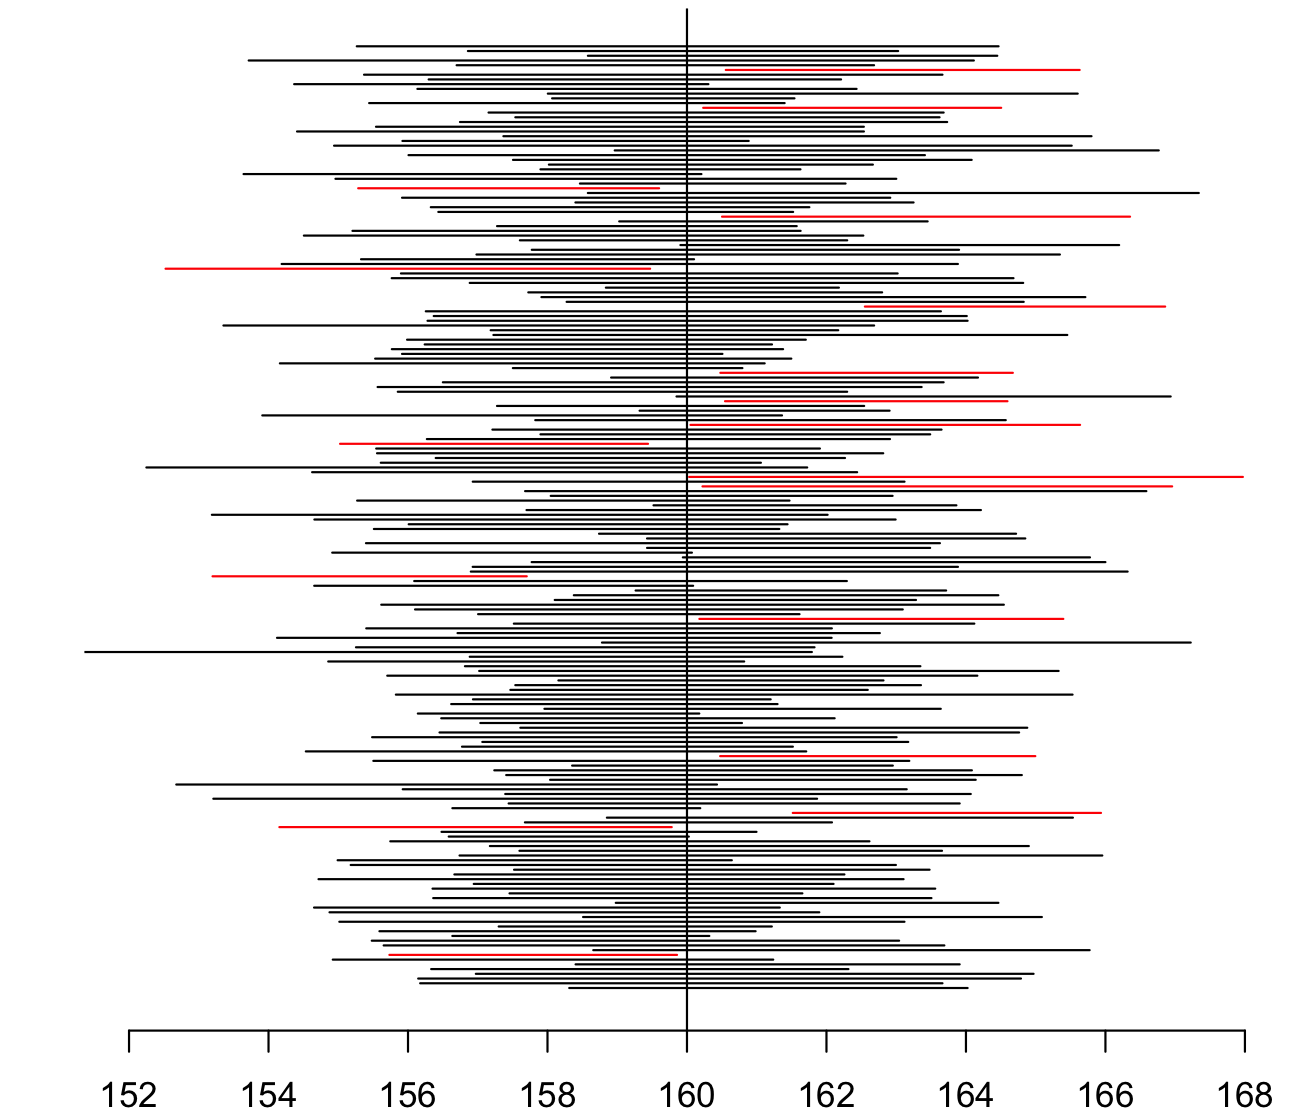
\includegraphics[width=0.7\textwidth]{figures/05-Confidence_interval/confidence_t.png}
        \caption{從 $\NN(160, 5^2)$ 抽出樣本數 9 的 200 組樣本所得的信賴區間(樣本標準差帶入母體標準差)}
        \label{fig:confidence_t}
    \end{figure}

    幸運的是,統計學家 William Gosset(1876—1937)在 1906 年初提出了一個新的分布,能夠幫助我們找出在這個情境中精確建構信賴區間的方法。Gosset 發現,若母體服從平均值為 $\mu$ 的常態分布,抽取樣本數為 $n$ 的樣本得到樣本平均 $\bar{X}$ 及樣本標準差 $s$,則
    \[\frac{\bar{X}-\mu}{s/\sqrt{n}} \sim t_{n-1}\]
    其中 $t_{n-1}$ 就是 Gosset 提出的 student $t$ 分布(這裡如果 $t$ 能夠大寫代表隨機變數的確比較不容易混淆,但是統計學界的習慣都寫小寫)。下標的 $n-1$ 是 $t$ 分布唯一的參數,被稱為\textit{自由度} (degrees of freedom)。這個自由度的由來可以看成是分母在計算樣本標準差時,使用的樣本數減去估計的參數個數,因此是 $n$ 個樣本減掉估計了一個樣本平均,總自由度為 $n-1$。$t$ 分布的機率密度函數如圖\ref{fig:student}所示。可以看到相對於標準常態分佈(黑色粗線) 而言,$t$ 分布的分布比較分散,雙尾比較厚重。但是隨著自由度 $\nu$ 上升,$t$ 分布的形狀會越來越接近標準常態分佈。事實上,當自由度 $\nu > 30$ 時,一般認為 $t$ 分布可以直接用標準常態分佈來近似。針對 $t$ 分布,我們也有 \href{https://en.wikipedia.org/wiki/Student%27s_t-distribution}{$t$分布表}可以查詢其曲線下面積。

    \begin{figure}[htbp]
        \centering
        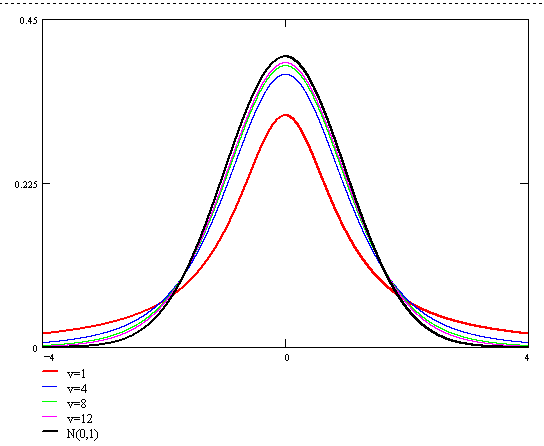
\includegraphics[trim={0 0 0 0.5cm},clip,width=0.7\textwidth]{figures/05-Confidence_interval/student.png}
        \caption{$t$分布的機率密度函數}
        \label{fig:student}
    \end{figure}

    回到我們建構信賴區間的目標,現在我們知道 $\frac{\bar{X}-\mu}{s/\sqrt{n}}$ 服從一個已知的 $t_{n-1}$ 分布,因此它又是一個樞紐量,我們可以參考前面的推導過程,先從以下的等式出發,建構出一個以 0 為中心左右對稱,且機率為 $(1-\alpha)\times 100\%$ 的區間:
     \[\PP(-t_{n-1, \alpha/2} < t_{n-1} < t_{n-1, \alpha/2}) = \alpha\]
    其中 $t_{\nu, p}$ 代表滿足 $\PP(t_{\nu} > t_{\nu, p}) = p$的數值,可以用查表得到。根據前面的分布,我們可以推出:
    \begin{align*}
        \PP\Big(-t_{n-1, \alpha/2} < \frac{\bar{X} - \mu}{s/\sqrt{n}} < t_{n-1, \alpha/2})\Big) &= \alpha\\
        \PP\Big(-t_{n-1, \alpha/2}\frac{s}{\sqrt{n}} < \bar{X} - \mu < t_{n-1, \alpha/2}\frac{s}{\sqrt{n}}\Big) &= \alpha\\
        \PP\Big(\bar{X}-t_{n-1, \alpha/2}\frac{s}{\sqrt{n}}< \mu < \bar{X} + t_{n-1, \alpha/2}\frac{s}{\sqrt{n}}\Big) &= \alpha\\
        \PP\Big(\mu \in \Big(\bar{X}-t_{n-1, \alpha/2}\frac{s}{\sqrt{n}},  \bar{X} + t_{n-1, \alpha/2}\frac{s}{\sqrt{n}}\Big)\Big) &= \alpha
    \end{align*}
    因此,母體為常態分布下的母體平均值 $(1-\alpha)\times 100\%$ 信賴區間可以寫為
    \[\Big(\bar{X}-t_{n-1, \alpha/2}\frac{s}{\sqrt{n}},  \bar{X} + t_{n-1, \alpha/2}\frac{s}{\sqrt{n}}\Big)\]
    可以看到,用 $t$ 分布建構的信賴區間和常態分布建構的信賴區間,基本上只差在臨界值改成查 $t_{n-1}$ 的表、以及標準差由母體標準差改為樣本標準差。前面我們提到 $t$ 分布都比標準常態分佈來得寬,所以 $t_{n-1, \alpha/2}$ 會比 $z_{\alpha/2}$ 來得大,也就是 $t$ 分布建構的信賴區間比常態分布建構的信賴區間來得寬。
    
    用類似的推導也可以得到右尾和左尾的 $(1-\alpha)\times 100\%$ 信賴區間分別可以寫為
    \[\Big(-\infty,  \bar{X} + t_{n-1, \alpha}\frac{s}{\sqrt{n}}\Big), \;\;\Big(\bar{X}-t_{n-1, \alpha}\frac{s}{\sqrt{n}},  \infty\Big)\]

    \bigskip

    \begin{custom}{練習}
        假設已知 60 歲以上國人血清低密度脂蛋白的濃度呈現常態分布。現隨機選取 16 位 60 歲以上的志願者抽血,得到血清低密度脂蛋白的平均濃度為 93 mg/dL,樣本標準差為 9 mg/dL。請問 60 歲以上國人平均血清低密度脂蛋白濃度的 (1) 雙尾 95\% 信賴區間為何? (2) 右尾 90\% 信賴區間為何?
    \end{custom}
    
    \begin{docexam}{(107-1醫學(二))}
        為了探討某社區之吸菸盛行狀況,由此社區隨機選取100位居民,發現其中30位居民具有吸菸習慣。在 5\% 的誤差水準下,此社區吸菸率的 95\% 信賴區間之上限值為何?
    \end{docexam} 
    
    \begin{docexam}{(103-1醫學(一))}
        對 100 名國小六年級學童量測體重,發現樣本平均值為 35 公斤,母群體平均值的 95\% 信賴區間為 33 公斤至 37 公斤。下列敘述何者正確?

        (A) 母群體平均值為 35 公斤

        (B) 該研究 100 名國小學童中,95 名的體重介在 33 至 37 公斤之間

        (C) 該樣本學童的體重標準差約 10 公斤

        (D) 若計算母群體平均值的 90 \% 信賴區間,其範圍會大於 95\% 信賴區間
    \end{docexam}